\section{The outgoing spectrum}\label{sec:spectrum}

Throughout this section, $Q=Ae^{i\phi}$ is one of the profiles of
Proposition~\ref{profile:existence}, and
\[
 P=A^{1/a},\quad \mu=A^2,\quad c_*=6-2a,\quad
 w=(r/2+2\phi')\partial_r,\quad W=w\cdot\nabla,\quad D=r\partial_r.
\]
The same letter $w$ denotes the radial component of the vector field when
it appears in a one-dimensional formula. Complexification is always
complexification of a real linear equation. Thus its two circular
components $v_+,v_-$ are independent; the original real space is the
subspace $v_- =\overline{v_+}$.

\begin{theorem}[Classification of regular modes]\label{spectrum:classification}
For all sufficiently small admissible $a>0$, the only regular outgoing
modes with $\operatorname{Re}\lambda\ge-1/32$ are the phase, translation,
and time modes. Their first circular components and eigenvalues are
\[
 iQ\quad(\lambda=0),\qquad
 \partial_jQ\quad(\lambda=1/2, 1\le j\le12),\qquad
 (a-ib+D/2)Q\quad(\lambda=1).
\]
The second component of each listed real symmetry generator is the
conjugate of the displayed component. Their complex spans are the
corresponding complexified eigenspaces. In
each fixed spherical harmonic, each eigenvalue that occurs is
algebraically simple; degrees $\ell\ge2$ have no such eigenvalue.

Here ``outgoing'' means that, in each component, for every fixed integer
$j\ge0$,
\begin{equation}\label{spec:slow-condition}
 D^jv_h=O(r^{-2(a+\operatorname{Re}\lambda)})\qquad(r\longrightarrow\infty).
\end{equation}
The same classification holds for regular solutions for which
$\partial_r^kv_h\in L^2(r^{11}\,dr)$ for some integer $k\ge7$.
There is no regular generalized mode above any of these eigenvectors
with this top-derivative integrability. Algebraic simplicity for
outgoing modes means simplicity of the analytic regular/outgoing
boundary problem, including its differentiated outgoing condition.
\end{theorem}

We prove the theorem in several steps. All statements about $a\to0$
allow a convergent subsequence of the profile parameters $(b,Z)$.
Uniform conclusions for all small $a$ will follow by contradiction and
subsequence extraction, so a continuous choice of matched profiles is
not needed.

\subsection{Linearization and the boundary condition at infinity}

Let a real spherical harmonic of degree $\ell$ have unit $L^2$ norm on
$\mathbb S^{11}$. Its eigenvalue for $-\Delta_{\mathbb S^{11}}$ is
$\ell(\ell+10)$. The mode equation in this harmonic is
\begin{equation}\label{spec:circular}
 v_h''+\left(\frac{11}{r}+\frac{hi r}{2}\right)v_h'
 +\left[b+hi(a+\lambda)-\frac{\ell(\ell+10)}{r^2}\right]v_h
 =Pv_h+\frac{P}{2a}(v_h+e^{2hi\phi}v_{-h}),\qquad h=\pm1.
\end{equation}
Set
\[
 v_h=Ae^{hi\phi}(f+hi g),\qquad X=(f,g)^t,
 \qquad J=\begin{pmatrix}0&1\\-1&0\end{pmatrix}.
\]
We include the angular harmonic in $f,g$ when using spatial notation.
The coordinates $f,g$ are independent complex variables in the spectral
problem and are real on the original real space.
Cancellation of the stationary profile terms gives
\begin{equation}\label{spec:real-system}
 \mathcal H X+J(\lambda+W)X=0,\qquad
 L=-\mu^{-1}\nabla\cdot(\mu\nabla),\qquad
 \mathcal H=\begin{pmatrix}L+P/a&0\\0&L\end{pmatrix}.
\end{equation}
Indeed the terms remaining after division by $Ae^{hi\phi}$ in
\eqref{spec:circular} are $-L+hiW$ and the additional pressure
$(P/a)f$. The evolutionary generator in these variables is therefore
$\mathcal G=J\mathcal H-W$. We use repeatedly
\begin{equation}\label{spec:divergence}
 \operatorname{div}(\mu w)=c_*\mu,
 \qquad W^*=-W-c_*
\end{equation}
in the weighted volume inner product, with the appropriate boundary
term on a ball.

\begin{lemma}[Block reduction at infinity]\label{spec:block-reduction}
Suppose that
\[
 DY=(r^2\Lambda(r)+B(r))Y
\]
on a half-line, where $\Lambda$ is diagonal, its selected blocks have
uniformly separated spectra, and $\Lambda,B$ and their fixed Euler
derivatives are bounded. For every fixed $m$ there is an invertible
change $I+O_m(r^{-2})$, with the same symbol bounds, after which the
off-block remainder is $O_m(r^{-m})$. The bounded part in each diagonal
block changes by $O_m(r^{-2})$. The changes preserve holomorphic
dependence on any parameters on which the original system depends
holomorphically.
\end{lemma}

\begin{proof}
Suppose an off-block entry is $b_{jk}=O(r^{-q})$. A change with entry
$-r^{-2}b_{jk}/(\Lambda_j-\Lambda_k)$ cancels it by commutation with
$r^2\Lambda$. Differentiating this change or multiplying it by the
bounded part gives $O(r^{-q-2})$; its products with the other changes
have the same or better order. The denominator and all its fixed
Euler derivatives are uniformly bounded by the spectral gap.
Perform this operation simultaneously on every off-block entry, and
iterate a finite number of times. The product of the changes is
invertible for sufficiently large $r$ by its $I+O_m(r^{-2})$ bound.
Differentiating the construction proves the symbol estimates. All
operations are algebraic operations and differentiation with nonzero
denominators, proving the last assertion.
\end{proof}

\begin{lemma}[Slow bases and exclusion of fast modes]\label{spec:slow-basis}
For bounded $\lambda,\ell$ and small $a$, the exterior solution space
of \eqref{spec:circular} has a two-dimensional outgoing subspace,
locally holomorphic in $\lambda$. Its bases and parameter derivatives
converge locally on $r\ge r_b$ to free outgoing bases as $a\to0$.
Every homogeneous solution satisfying the top-derivative condition
in Theorem~\ref{spectrum:classification} belongs to this subspace.
\end{lemma}

\begin{proof}
Use $(v_h,v_h'/r)$ for each channel. The coefficient of $r^2$ in its
$D$ equation is
\[
 \begin{pmatrix}0&1\\0&-hi/2\end{pmatrix}.
\]
Diagonalize by the eigenvectors with first component one, group the
two zero eigenvalues, and apply Lemma~\ref{spec:block-reduction}.
Writing
\[
 \nu_h=-2(a+\lambda)+2hib,
\]
the slow block is $\operatorname{diag}(\nu_h)+O(r^{-2})$, and the fast
entries are $-hi r^2/2-12-\nu_h+O(r^{-2})$.
For example, before diagonalization the bounded contribution to the
second row is $-12(v_h'/r)-(b+hi(a+\lambda))v_h$; this verifies both
constant exponents.

Factor out $r^{\nu_h}$ in a slow coordinate and
$e^{-hi r^2/4}r^{-12-\nu_h}$ in a fast coordinate. The diagonal errors
are integrable in $d r/r$. The off-block errors are also integrable if
$m>|12+2\operatorname{Re}\nu_h|$ with a fixed positive margin on the
parameter neighborhood. The factored equation is thus an integrable
perturbation of a constant vector. On a sufficiently late half-line,
its integral from infinity is a contraction on bounded vectors;
prescribing its four limits gives four independent solutions.
Continuation gives a basis on the entire exterior. This construction
is holomorphic on a slightly smaller parameter neighborhood because
the integrable majorants are uniform there.

Setting both fast limits to zero gives exactly the outgoing subspace.
In fact the fast coordinates forced by slow coordinates are
$O(r^{\operatorname{Re}\nu_h-m})$ before factoring, by the backward
integral. Taking $m$ larger before each fixed number of differentiations
gives \eqref{spec:slow-condition}. Increasing the reduction order does
not change the limiting normalization: the additional transformations
have arbitrarily high order relative to the prescribed normalization,
and uniqueness of the backward integral applies on a common tail.
Uniform exterior symbol bounds for the profiles and their convergence
give convergence of these integral equations by dominated convergence;
ordinary ODE continuation then proves the asserted local convergence.
At $a=0$ the slow columns are, up to their nonzero normalizations,
\begin{equation}\label{spec:free-bases}
 r^\ell H(\lambda+\ell/2-hib,6+\ell,-hi r^2/4)
\end{equation}
in their separate channels, by Lemma~\ref{free:slow}.

If the fast limit $d_h$ in channel $h$ is nonzero, reconstruction and
$k$ radial differentiations give the leading fast term
\begin{equation}\label{spec:fast-derivative}
 \partial_r^k v_h=
 (-hi/2)^k e^{-hi r^2/4}r^{k-12-\nu_h}(d_h+o(1))
 +O(r^{\operatorname{Re}\nu_h-k}).
\end{equation}
The other channel's fast contribution is smaller by $r^{-2}$; this
follows from the off-block reconstruction. The same formula follows
directly by successively applying $D$ to the reduced fast equation,
whose leading multiplier is $-hi r^2/2$.
For $\operatorname{Re}\lambda\ge-1/32$ and $k\ge7$,
$2k>12+2\operatorname{Re}\nu_h$. Consequently the first term in
\eqref{spec:fast-derivative} dominates the slow term and its square is
not integrable against $r^{11}\,dr$. Thus every fast limit vanishes.
For any particular finite $\lambda,\ell$, the argument applies in a
bounded neighborhood of those parameters; it does not require a
uniform bound on the parameters of the mode being tested.
\end{proof}

\begin{lemma}[Upper bound for the real part]\label{spec:real-bound}
For all sufficiently small $a$, there is no nonzero regular outgoing
mode with $\operatorname{Re}\lambda\ge4$.
\end{lemma}

\begin{proof}
Put $V_a=P/a$ and $\sigma=\operatorname{Re}\lambda$. Test
\eqref{spec:real-system} against $(\lambda+W)X$, and take real parts.
The $J$ term has zero real part. Integration by parts, using
\eqref{spec:divergence}, gives
\begin{equation}\label{spec:upper-energy}
 0=\int\left\{(\sigma-c_*/2)(|\nabla X|^2+V_a|f|^2)
 +\nabla X^*(\nabla w)\nabla X
 -\tfrac12 W(V_a)|f|^2\right\}\mu\,dy.
\end{equation}
Here the matrix $\nabla w$ acts on spatial indices and the expression
is summed over the two components. Boundary terms vanish: after
division by $A$, the slow bound is $X=O(r^{-2\sigma})$, with its symbol
derivatives, and $\sigma\ge4$ gives all needed integrability.

For completeness, the weighted Hardy inequality used here is uniform
for small $a$:
\begin{equation}\label{spec:hardy}
 \int r^{-2}|f|^2\mu\,dy\le C\int|\nabla f|^2\mu\,dy.
\end{equation}
Indeed, for $\rho=\langle r\rangle^{-4a}$,
$\operatorname{div}(\rho y/r^2)\ge(10-4a)\rho/r^2$.
Integration against $|f|^2$ and Cauchy--Schwarz prove the inequality
with $\rho$; comparability of $\rho$ and $\mu$ proves
\eqref{spec:hardy}. Cutoffs justify the calculation by density.
Proposition~\ref{profile:existence} gives $\nabla w\ge cI$ and
$W(V_a)\le C a V_a$ on the inner ball, while its exterior positive
part is $o(1)r^{-2}$. Since $\sigma-c_*/2\ge1$, these two negative
contributions in \eqref{spec:upper-energy} are absorbed, respectively,
by the pressure and gradient terms. A nonzero $X$ is impossible.
\end{proof}

\subsection{An outgoing estimate for unbounded parameters}

We next exclude loss of modes to large angular or imaginary spectral
parameters. The main step is to express the outgoing condition as a relation
between a mode and its radial derivative on one fixed exterior shell.
Once this relation is available, interior energy and flux identities will
exclude a regular mode. Consider a sequence with $a\to0$,
$-1/32\le\sigma\le4$, and
$\ell+|\operatorname{Im}\lambda|\to\infty$. Complex conjugation of
\eqref{spec:real-system} allows us to assume
$\omega=\operatorname{Im}\lambda\ge0$. After extraction, one of the
following holds:
\begin{equation}\label{spec:cases}
 \text{I: }\frac{\ell}{\sqrt{1+\omega}}\longrightarrow\infty;
 \qquad
 \text{II: }\omega\longrightarrow\infty,\quad
 \frac{\ell}{\sqrt\omega}\text{ is bounded}.
\end{equation}
Set
\begin{equation}\label{spec:high-definitions}
 \begin{split}
 q_h&=r^{11/2}e^{hi r^2/8}v_h,\qquad
 L_\ell=(\ell+5)^2-\tfrac14,\qquad n_* =\max(1+\ell,\sqrt\omega),\\
 F_h&=r^2/16+b-h\omega-L_\ell/r^2,
 \qquad S=\max(1+\ell,\omega),\qquad E=16\sqrt S.
 \end{split}
\end{equation}
The symbol $q_h$ here denotes an unknown function, not the first
argument of $H$. Direct substitution gives
\begin{equation}\label{spec:schrodinger-radial}
 q_h''+(F_h+hi\gamma)q_h=\sum_j V_{hj}(r)q_j,
 \qquad \gamma=\sigma+a-3,\qquad |V_{hj}(r)|\le Cr^{-2}
 \quad(r\ge r_b).
\end{equation}
The bound, uniform in the sequence, follows from the exterior pressure
estimates; oscillations in $V_{hj}$ cause no difficulty below.

Choose a fixed $B_0>r_b$, and put $B_1=B_0+1$. In Case II take $B_0$
large enough that $L_\ell/B_0^2<\omega/2$ eventually. On this shell
$F_h<0$ for both channels in Case I; in Case II $F_+<0<F_-$.
In either case $|F_h|\asymp n_*^2$, uniformly on the shell.

\begin{lemma}[Outgoing data at the remote endpoint]\label{spec:remote-data}
Every outgoing solution along this sequence satisfies
\begin{equation}\label{spec:remote-robin}
 q_h'(E)-hi\sqrt{F_h(E)}q_h(E)=O(E^{-1})|q(E)|.
\end{equation}
The constant is uniform after discarding finitely many sequence terms.
\end{lemma}

\begin{proof}
For $r\ge E$ use $(v_h,v_h'/r)$ again. Diagonalize the leading matrix
\[
 \begin{pmatrix}
 0&1\\ h\omega/r^2+\ell(\ell+10)/r^4&-hi/2
 \end{pmatrix}.
\]
Its eigenvalues are
\[
 hi\left(-\tfrac14\pm
 \sqrt{\tfrac1{16}-h\omega/r^2-\ell(\ell+10)/r^4}\right).
\]
The square root stays uniformly positive on $r\ge E$. Eigenvectors
with first entry one give a uniformly invertible symbol change.
Group the two plus signs as the outgoing block; take the two minus
signs as separate blocks. These blocks have uniformly positive gaps.
The bounded remainder has norm at most a fixed $C_0$, with uniform
fixed symbol derivatives. The leading diagonal is purely imaginary.

The order of choices is important. First choose $C>C_0+2$, enlarged
if necessary to bound the Hermitian parts of the initial full and
block systems. Next choose one fixed integer $m>2C+4$. Apply
Lemma~\ref{spec:block-reduction} to this order. Finally pass far enough
along the sequence that its finitely many $O_m(r^{-2})$ corrections
have norm at most one on $r\ge E$. Both the full reduced evolution
and each block evolution then have propagator bound
\begin{equation}\label{spec:power-propagator}
 \|\Phi(r,t)\|\le
 \left(\frac{\max(r,t)}{\min(r,t)}\right)^C.
\end{equation}
This is Gronwall in $\log r$ after using skewness of the leading
diagonal. No separation inside the outgoing block is required.

For each individual outgoing solution, all reduced coordinates have
symbol bounds $O(r^\rho)$, where $\rho=-2(a+\sigma)<1$; their constants
may depend on that solution and its parameters. In an incoming
equation the $r^2$ leading coefficient is invertible. Solving for that
coordinate and differentiating gives a gain of two powers of $r$;
iteration gives the same gain for each fixed symbol derivative, up
to the $O_m(r^{-m})$ forcing from the outgoing block. Thus the incoming
coordinate is $o(r^{-C-1})$, with $m$ as chosen. This qualitative
bound is used only to remove its terminal value in variation of
constants at infinity.

After that terminal value has vanished, the quantitative estimate
uses only \eqref{spec:power-propagator}. If $Y$ denotes all reduced
coordinates, its incoming part at $E$ is at most
\[
 C_m|Y(E)|\int_E^\infty(r/E)^{2C}r^{-m}\frac{dr}{r}
 =\frac{C_mE^{-m}}{m-2C}|Y(E)|.
\]
Undoing the changes gives
\[
 \frac{v_h'(E)}E=
 hi\left(-\tfrac14+
 \sqrt{\tfrac1{16}-h\omega/E^2-\ell(\ell+10)/E^4}\right)v_h(E)
 +O(E^{-2})|v(E)|.
\]
The full coordinate size is bounded by $C|v(E)|$, since the incoming
coordinates are small and the first entry of each outgoing
eigenvector is one. Multiplication by the scalar defining $q_h$
proves \eqref{spec:remote-robin}; the $11/(2E)$ term and the difference
between $L_\ell$ and $\ell(\ell+10)$ are within its error.
\end{proof}

\begin{lemma}[Scalar transfer and a turning point]\label{spec:scalar-turn}
Fix one channel and write $F=F_h$. For $R\in[B_0,B_1]$, let $U$ solve
\[
 U''+(F+hi\gamma)U=0,\qquad
 U(E)=F(E)^{-1/4},\quad U'(E)=hi\sqrt{F(E)}U(E).
\]
If $F$ has a zero $r_0\in[R,E]$, define
\begin{equation}\label{spec:turn-scales}
 \begin{split}
 A_0&=r_0^2/16,\qquad H_0=L_\ell/r_0^2,\qquad k_0^2=A_0+H_0,\\
 d_0&=(r_0/(2k_0^2))^{1/3},\qquad
 K(r)=(|F(r)|+d_0^{-2})^{1/2},\\
 H_f(r)&=\int_{\min(r,r_0)}^{r_0}\sqrt{-F(t)}\,dt.
 \end{split}
\end{equation}
If there is no zero, put $K=\sqrt F$ and $H_f=0$.
For $N_r(u)=K(r)^{1/2}|u(r)|+K(r)^{-1/2}|u'(r)|$, after taking a
subsequence common to the two channels, there are $c,C>0$ such that
\begin{align}
 N_r(u)&\le C e^{|H_f(r)-H_f(t)|}N_t(u),\label{spec:scalar-transfer}\\
 |U(R)|&\ge cK(R)^{-1/2}e^{H_f(R)},\label{spec:scalar-value}\\
 U'(R)/U(R)&=\mathcal B_h(R)+o(n_*),\label{spec:scalar-slope}
 \end{align}
where
\[
 \mathcal B_h(R)=
 \begin{cases}-\sqrt{-F_h(R)},&F_h(R)<0,\\
 hi\sqrt{F_h(R)},&F_h(R)>0.
 \end{cases}
\]
The first estimate holds for every scalar homogeneous solution and
all $r,t\in[R,E]$. All left endpoint statements are uniform for
$R\in[B_0,B_1]$.
\end{lemma}

\begin{proof}
The derivative $F'=r/8+2L_\ell/r^3$ is positive, so there is at most
one zero. In the turning cases its defining equation gives
\begin{equation}\label{spec:turn-potential}
 F(r)=A_0((r/r_0)^2-1)+H_0(1-(r_0/r)^2),\qquad
 A_0-H_0=h\omega-b.
\end{equation}
It follows that $k_0^2\asymp S$, $r_0\to\infty$, $r_0<E/2$, and
$d_0\to0$. For the $h=-1$ turn in Case I, for example,
$r_0^2\asymp \ell^2/(\omega+\ell)$, which tends to infinity precisely
because $\ell/\sqrt{1+\omega}\to\infty$. The other turn has
$r_0^2\asymp\omega+\ell$. In the no-turn case, necessarily the
negative channel in Case II, $F\asymp S$ throughout $[R,E]$.

Fix a large number $M$ and remove the interval $|r-r_0|<Md_0$.
On either remaining interval choose $\operatorname{Re}p>0$ with
$p^2=\operatorname{sign}(F)(F+hi\gamma)$. Use the two approximate
solutions
\[
 p^{-1/2}\exp(\pm\!\int p)\quad(F<0),\qquad
 p^{-1/2}\exp(\pm i\!\int p)\quad(F>0).
\]
All integrals in this paragraph are over the outer intervals. Direct
differentiation of \eqref{spec:turn-potential} gives
\begin{align}
 \int |F|^{-1/2}\,dr&\le C,\label{spec:phase-error}\\
 \sup\frac{|F'|}{|F|^{3/2}}+
 \int\left(\frac{|F''|}{|F|^{3/2}}
       +\frac{|F'|^2}{|F|^{5/2}}\right)dr
 &\le CM^{-3/2}+o(1).\label{spec:wkb-error}
\end{align}
Here and below the constants multiplying $M^{-3/2}$ do not depend on
$M$. To verify the estimates, on $[r_0/2,2r_0]$ use
$|F|\asymp k_0^2|r-r_0|/r_0$,
$|F'|\le Ck_0^2/r_0$, $|F''|\le Ck_0^2/r_0^2$ and
$d_0^3=r_0/(2k_0^2)$. Integrating the powers
$|r-r_0|^{-3/2}$ and $|r-r_0|^{-5/2}$ from $Md_0$ gives the stated
error. Off this interval $|F|\gtrsim k_0^2$, with relative derivative
bounds $C/r,C/r^2$, and $E\lesssim k_0$; splitting at $r_0/2$ and
$2r_0$ gives a vanishing error and the bounded integral in
\eqref{spec:phase-error}. For no turn the same computations use
$F\asymp S$ and give $o(1)$ in \eqref{spec:wkb-error} on all of $[R,E]$.

Here is a transfer justification retaining the error that will be
needed below. Each approximate solution has residual potential
\[
 \frac{(p^{-1/2})''}{p^{-1/2}}
 =\frac34(p'/p)^2-\frac12p''/p.
\]
The approximate pair has constant nonzero Wronskian. Its transfer
matrix in the $N$ norms is at most
$C\exp(|H_f(r)-H_f(t)|)$: $K\asymp|p|$, and
$\int|p-\sqrt{|F|}|\,dr\le C$ by \eqref{spec:phase-error}.
Variation of constants for the residual followed by Gronwall bounds
the difference between exact and approximate transfer by
\begin{equation}\label{spec:transfer-error}
 (CM^{-3/2}+o(1))e^{|H_f(r)-H_f(t)|}.
\end{equation}
Indeed the residual divided by $K$ has integral bounded by
\eqref{spec:wkb-error}; when $r,s,t$ occur in order, monotonicity of
$H_f$ gives
$|H_f(r)-H_f(s)|+|H_f(s)-H_f(t)|=|H_f(r)-H_f(t)|$.
This removes the exponential factor from the integral inequality.
With no turn the error coefficient is $o(1)$.

At $E$, the prescribed data select the outgoing approximate branch
up to an error tending to zero. On the positive outer interval,
\eqref{spec:phase-error} bounds its normalized amplitude above and
below, because the absolute imaginary action is bounded. Consequently
\begin{equation}\label{spec:positive-branch}
 c\le F^{1/4}|U|\le C,\qquad
 \frac{U'}{\sqrt F\,U}=hi+O(M^{-3/2})+o(1).
\end{equation}
This proves all claims in the no-turn case.

In a turning case set $\xi=(r-r_0)/d_0$ and
$Y(\xi)=d_0^{-1/2}U(r_0+d_0\xi)$. Since
$F'(r_0)d_0^3=1$ and $\gamma d_0^2\to0$, its equation converges on
every fixed $\xi$ interval to
\begin{equation}\label{spec:airy-equation}
 Y_\infty''+\xi Y_\infty=0.
\end{equation}
The corresponding transfer on $[-M,M]$ is bounded in the scaled data
norm, with a bound depending only on fixed $M$.
Figure~\ref{fig:turning} records these three regions.
\begin{figure}[tbp]
  \centering
  \begingroup
  \definecolor{turnblue}{RGB}{48,91,120}
  \definecolor{turnorange}{RGB}{163,92,43}
  \resizebox{0.95\linewidth}{!}{%
  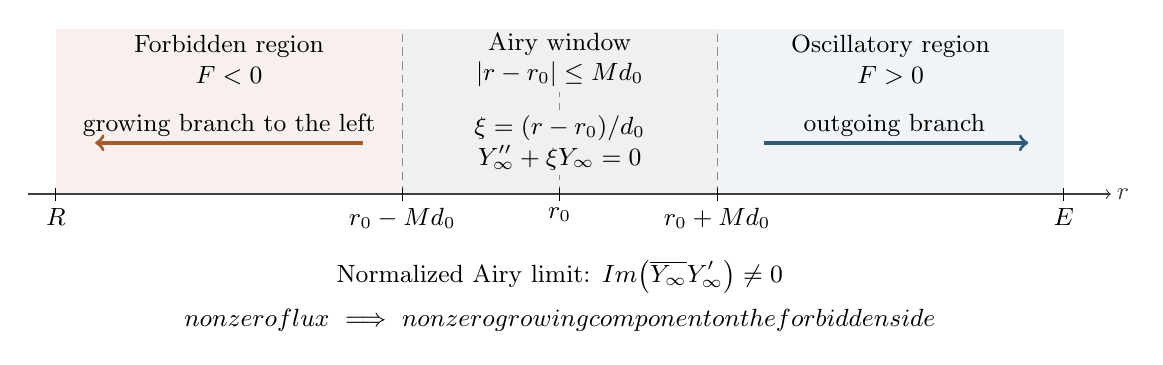
\begin{tikzpicture}[
    x=1cm,y=1cm,font=\small,
    guide/.style={densely dashed,thin,black!45},
    every node/.style={inner sep=2pt}]
    \fill[turnorange!9] (.6,0) rectangle (5,2.1);
    \fill[black!6] (5,0) rectangle (9,2.1);
    \fill[turnblue!7] (9,0) rectangle (13.4,2.1);
    \draw[guide] (5,0) -- (5,2.1);
    \draw[guide] (9,0) -- (9,2.1);
    \draw[guide] (7,0) -- (7,1.3);
    \node[align=center] at (2.8,1.7) {Forbidden region\\$F<0$};
    \node[align=center] at (7,1.7) {Airy window\\$|r-r_0|\le M d_0$};
    \node[align=center] at (11.2,1.7) {Oscillatory region\\$F>0$};
    \draw[<-,very thick,turnorange] (1.1,.65) -- (4.5,.65);
    \node[above] at (2.8,.65) {growing branch to the left};
    \node[align=center,fill=black!6] at (7,.65) {$\xi=(r-r_0)/d_0$\\$Y_\infty''+\xi Y_\infty=0$};
    \draw[->,very thick,turnblue] (9.6,.65) -- (12.95,.65);
    \node[above] at (11.25,.65) {outgoing branch};
    \draw[->,thin,black!75] (.25,0) -- (14,0) node[right] {$r$};
    \foreach \x in {.6,5,7,9,13.4}
      \draw (\x,.08) -- (\x,-.09);
    \node[below] at (.6,-.1) {$R$};
    \node[below] at (5,-.1) {$r_0-Md_0$};
    \node[below] at (7,-.1) {$r_0$};
    \node[below] at (9,-.1) {$r_0+Md_0$};
    \node[below] at (13.4,-.1) {$E$};
    \node[align=center] at (7,-1.05)
      {Normalized Airy limit: $\displaystyle
       \operatorname{Im}\!\left(\overline{Y_\infty}Y_\infty'\right)\ne0$};
    \node[align=center] at (7,-1.6)
      {$\text{nonzero flux}\ \Longrightarrow\ \text{nonzero growing component on the forbidden side}$};
  \end{tikzpicture}%
  }
  \endgroup
  \caption{Schematic of a channel with one turning point in the
  high-parameter estimate, with $R\in[B_0,B_1]$ as in
  Lemma~\ref{spec:scalar-turn}. The scalar solution is selected at $E$ by
  $U(E)=F(E)^{-1/4}$ and $U'(E)=h i\sqrt{F(E)}\,U(E)$.
  For a fixed large $M$, pass to a subsequence and take the
  high-parameter limit in the window using $Y=d_0^{-1/2}U$
  and $\xi=(r-r_0)/d_0$.
  The resulting Airy solution has constant nonzero flux, so it contains
  a branch growing towards $R$.
  Only after this fixed-window limit is $M$ allowed to tend to infinity
  to obtain the normalized logarithmic derivative
  $U'(R)/(\sqrt{-F(R)}\,U(R))\to-1$.
  Distances are not to scale, and the arrows indicate branch selection,
  not a graph of $U$ or a sign assertion for its complex values.}
  \label{fig:turning}
\end{figure}


Choose one fixed $M_0$ so large that the error in
\eqref{spec:positive-branch} is below its lower amplitude margin.
At $\xi=M_0$, the scaled Cauchy data are bounded and their flux
\[
 \operatorname{Im}(\overline Y Y')
 =\operatorname{Im}(\overline U U')
\]
has sign $h$ and magnitude bounded below. A subsequence of these data
converges, and continuous dependence of the scaled ODE gives one
solution $Y_\infty$ on every fixed interval. Its flux is nonzero and
constant, since \eqref{spec:airy-equation} has real coefficients.

We spell out why this gives the required \emph{relative} margin on
the forbidden side. With $t=-\xi$, the real equation is $y''-ty=0$.
On a sufficiently late half-line it has a positive growing solution
comparable to $t^{-1/4}\exp(2t^{3/2}/3)$. To construct one, prescribe
the growing approximate data at a fixed large $T$ and use the residual
transfer estimate with $p=\sqrt t$: the total error relative to the
growing scale is at most $CT^{-3/2}$. The exact solution and its
derivative are positive when $T$ is large. Its logarithmic slope
$z=y'/(\sqrt t\,y)$ satisfies
\[
 z'=\sqrt t(1-z^2)-\frac{z}{2t}.
\]
This equation implies $z\to1$: for every fixed $\epsilon>0$, its
derivative points into $[1-\epsilon,1+\epsilon]$ at both endpoints
for sufficiently large $t$, and outside that interval it points
inwards with magnitude bounded below by a positive multiple of
$\sqrt t$. A decaying independent solution is obtained by multiplying
the growing one by $\int_t^\infty y(s)^{-2}\,ds$. The growing
comparison bound makes that integral finite and shows that this
second solution and its derivative are negligible relative to the
first. These real solutions have nonzero Wronskian. A complex multiple
of the decaying solution alone has zero flux. Thus the coefficient of
the growing solution in $Y_\infty$ is nonzero.

As $M\to\infty$ its growing contribution dominates its decaying one,
and
\[
 \frac{Y_\infty'(-M)}{\sqrt M\,Y_\infty(-M)}\longrightarrow-1.
\]
In the approximate basis referenced at $r_-=r_0-Md_0$, the coefficient
of growth to the left therefore has magnitude at least a fixed
positive fraction of $N_{r_-}(U)$, for every sufficiently large fixed
$M$ and subsequently late sequence indices. That fraction can be
chosen independently of $M$: the normalized basis vectors have
comparable size one at their reference point, and the displayed
slope is separated from the decaying slope $+1$. For each such fixed
$M$, $N_{r_-}(U)$ is also bounded below by a positive constant.

Transfer to $R$ now gives a growing term of size at least
$cN_{r_-}(U)e^{H_f(R)-H_f(r_-)}$; the decaying term is negligible since
the action difference tends to infinity. The transfer error
\eqref{spec:transfer-error}, relative to this growing term, is still
$CM^{-3/2}+o(1)$ with $C$ independent of $M$, precisely because of the
relative coefficient margin. For the value lower bound, choose one
sufficiently large fixed $M$ and retain it; then $H_f(r_-)=O_M(1)$
and \eqref{spec:scalar-value} follows with a positive constant.
For the slope take an arbitrary sufficiently large fixed $M$, obtain
error $CM^{-3/2}+o(1)$, and then let $M\to\infty$. This proves
\eqref{spec:scalar-slope}. The transfer estimate follows from the two
outer estimates and the scaled central transfer, using one fixed
$M$. Both channels can use a common extracted subsequence. Finally,
all estimates allow a moving $R$ in the fixed shell, where
$|F_h(R)|\asymp n_*^2$. If uniformity there failed, the same argument
at a sequence of offending endpoints would contradict the estimates.
\end{proof}

\begin{lemma}[Coupled outgoing data on a fixed shell]\label{spec:boundary-estimate}
After subselection, every outgoing solution along an escaping
parameter sequence satisfies, uniformly on $B_0\le R\le B_1$,
\begin{equation}\label{spec:shell-robin}
 q_h'(R)=\mathcal B_h(R)q_h(R)+o(n_*)|q(R)|.
\end{equation}
The error is an operator bound on the two-dimensional outgoing space.
\end{lemma}

\begin{proof}
For each scalar channel let $D_h(R)=0$, $D_h'(R)=K_h(R)^{1/2}$.
Lemma~\ref{spec:scalar-turn} gives
\[
 N_r(D_h)\le Ce^{H_h(R)-H_h(r)},\quad
 N_r(U_h)\le Ce^{H_h(r)},\quad
 |\mathcal W(D_h,U_h)|\ge ce^{H_h(R)},
\]
where $H_h=H_f$ in that channel. The Green kernel with left
Dirichlet data and the right Robin condition of $U_h$ is the product
of $D_h$ on the left and $U_h$ on the right, divided by the Wronskian.
It obeys the following two different action bounds:
\begin{equation}\label{spec:green-actions}
 N_r(G_h(r,t))\le C K_h(t)^{-1/2}
 \begin{cases}
 e^{H_h(t)-H_h(r)},&r<t,\\
 e^{H_h(r)-H_h(t)},&r>t.
 \end{cases}
\end{equation}
Each exponential is at most one, by monotonicity within its own
channel. There is no comparison of $H_+$ and $H_-$. A right Robin
derivative error $\beta_h$, with zero left data, similarly gives
$N_r\le CK_h(E)^{-1/2}|\beta_h|$; this follows either from the same
Wronskian or by using $D_h$ for the correction.

Let $\kappa=\min_{h,r\in[R,E]}K_h(r)$. Then $\kappa\to\infty$:
at a turn it is $d_0^{-1}$, and in the no-turn case it is comparable
to $\sqrt S$. Put $\mathcal N(q)=\max_h\sup_rN_r(q_h)$.
The matrix forcing in \eqref{spec:schrodinger-radial} has Green norm
at most
\begin{equation}\label{spec:coupling-norm}
 C\max_{h,j}\int_R^E
 \frac{t^{-2}\,dt}{\sqrt{K_h(t)K_j(t)}}
 \le\frac{C}{R\kappa}=o(1).
\end{equation}
Also $K_h(E)\asymp E$ for both channels, so the right error
\eqref{spec:remote-robin} has norm at most $CE^{-2}\mathcal N(q)$.
The diagonal outgoing extension
$q_h(R)U_h(r)/U_h(R)$ has norm at most
$Cn_*^{1/2}|q(R)|$, since $K_h(R)\asymp n_*$ and
$H_h(r)\le H_h(R)$. Variation of constants and absorption of
\eqref{spec:coupling-norm} and the Robin error give
\[
 \mathcal N(q)\le Cn_*^{1/2}|q(R)|,\qquad
 \mathcal N\left(q-\left(q_h(R)U_h/U_h(R)\right)_h\right)
 =o(1)n_*^{1/2}|q(R)|.
\]
Taking the derivative at $R$ costs $K_h(R)^{1/2}\asymp n_*^{1/2}$.
Together with \eqref{spec:scalar-slope}, this is
\eqref{spec:shell-robin}. Every estimate used is homogeneous in the
left data and uniform over the shell.
\end{proof}

\begin{lemma}[Exclusion of escaping parameters]\label{spec:high-exclusion}
There is no sequence of nonzero regular outgoing modes with $a\to0$,
$-1/32\le\operatorname{Re}\lambda\le4$, and
$\ell+|\operatorname{Im}\lambda|\to\infty$.
\end{lemma}

\begin{proof}
Use \eqref{spec:cases} and Lemma~\ref{spec:boundary-estimate}.
All volume pairings in this proof have weight $\mu$, and $[\cdot]$
denotes its surface integral at the current sphere, including the
factor $r^{11}$. On a fixed ball $\mu$ is uniformly bounded above and
below, and the coefficients of $W$ and $L+\Delta$ are uniformly
bounded.

In Case I pair \eqref{spec:real-system} with $X$ on the ball $r<B_1$
and take real parts. The second-order term is
\[
 \int(|\nabla X|^2+(P/a)|f|^2)\mu-\operatorname{Re}[X^*X'].
\]
The boundary term has nonpositive real part, by
\eqref{spec:shell-robin} and both negative signs of $F_h$.
More precisely its real part is
$\frac12\operatorname{Re}\sum_h\overline q_hq_h'+O(|q|^2)$, so its
leading value is $-c n_*|q|^2$ and absorbs its errors.
The absolute value of the remaining real terms is at most
$C\|X\|_2\|\nabla X\|_2+C(1+\omega)\|X\|_2^2$.
The angular barrier
\[
 \|\nabla X\|_2^2\ge
 \ell(\ell+10)B_1^{-2}\|X\|_2^2
\]
and $\omega=o(\ell^2)$ absorb these terms into an arbitrarily small
fraction of the gradient term. Nonnegative pressure then gives a
contradiction.

In Case II normalize
\begin{equation}\label{spec:case-II-normalization}
 \int_{r<B_1}(|X|^2+|\nabla X|^2)\mu=1.
\end{equation}
Write the shell error in \eqref{spec:shell-robin} as
$\varepsilon n_*|q|$, with $\varepsilon\to0$. Its leading diagonal
has modulus at least $c n_*$, so $n_*|q|\le C|q'|$ on the shell.
There is a point in its first half at which both $|q'|$ and
$n_*|q|$ are bounded, by the shell integral bound furnished by
\eqref{spec:case-II-normalization}.
For the channel $h=-1$, the energy
$|q_-'|^2+F_-|q_-|^2$ propagates this bound to $B_1$.
Indeed $|F_-'|/F_-\le C$, $F_-\asymp n_*^2$ on the shell, and the
forcing in its equation has bounded integral, since it is at most
$C|q|$ there. Differentiating the square root of this energy and
applying Gronwall proves
\[
 |q_-'|+n_*|q_-|\le C
\]
from that point to $B_1$.
The positive channel then obeys, in the upper-derivative sense,
\[
 \frac{d}{dr}|q_+|
 \le-(\sqrt{-F_+}-\varepsilon n_*)|q_+|+C\varepsilon.
\]
The distance from the chosen point to $B_1$ is at least $1/2$.
Integrating this inequality with $\sqrt{-F_+}\ge c n_*$ gives
\begin{equation}\label{spec:plus-vanishing}
 n_*q_+(B_1)\longrightarrow0,\qquad q_+'(B_1)\longrightarrow0.
\end{equation}

We next remove the other boundary channel by a flux identity.
The imaginary part of the pairing of \eqref{spec:real-system} with
$X$ is
\begin{equation}\label{spec:flux}
 \operatorname{Im}[X^*X']
 =\frac{w(B_1)}2\operatorname{Im}[X^*JX]
 +(\sigma-c_*/2)\int\operatorname{Im}(X^*JX)\mu.
\end{equation}
To check the first-order term, integration by parts and
\eqref{spec:divergence} give
\[
2\operatorname{Im}\int X^*JW X\,\mu
=w(B_1)\operatorname{Im}[X^*JX]-c_*\int\operatorname{Im}(X^*JX)\mu.
\]
Also the pressure-free equation $Lg=(\lambda+W)f$, tested against $g$,
gives
\begin{equation}\label{spec:cross-small}
 \left|\int\overline g f\,\mu\right|\le C/\omega.
\end{equation}
Its integrated gradient term, $W$ term, and boundary term are bounded
by the normalization and the boundary bounds already obtained.
The change to circular coordinates gives the exact cancellation
\[
 \operatorname{Im}[X^*X']
 -\frac{w(B_1)}2\operatorname{Im}[X^*JX]
 =\frac12\sum_h\operatorname{Im}(\overline q_hq_h')(B_1).
\]
Multiplying \eqref{spec:flux} by $n_*\asymp\sqrt\omega$, and using
\eqref{spec:cross-small}, makes its right volume term tend to zero.
The positive channel contributes $o(1)$ by
\eqref{spec:plus-vanishing}. The outgoing relation for the other
channel gives
$\operatorname{Im}(\overline q_-q_-')=-\sqrt{F_-}|q_-|^2+
o(n_*)|q_-||q|$. Its sign and $F_-\asymp n_*^2$ imply
\begin{equation}\label{spec:all-boundary-small}
 n_*|q(B_1)|+|q'(B_1)|\longrightarrow0.
\end{equation}

Rellich compactness on the ball, including the full angular fields,
gives a strongly $L^2$ convergent subsequence of $f$. The equation
$Lg-Wf=\lambda f$ has uniformly bounded left side in $H^{-1}$ by
the normalization. Division by $\lambda$, whose modulus tends to
infinity, shows that the limit is zero. Thus
\begin{equation}\label{spec:f-small}
 f\longrightarrow0\quad\hbox{strongly in }L^2(r<B_1).
\end{equation}

Finally put $S_d=W+c_*/2$ and test \eqref{spec:real-system} against
$S_dX$. The real part of the second-order and pressure terms is
\begin{align*}
 &\int\left(\nabla X^*(\nabla w)\nabla X
       -\tfrac12W(P/a)|f|^2\right)\mu\\
 &\hspace{8mm}
 +\frac{w(B_1)}2[|\nabla X|^2+(P/a)|f|^2]
 -\operatorname{Re}[(S_dX)^*X'].
\end{align*}
All boundary terms vanish by \eqref{spec:all-boundary-small}; the
tangential derivatives cost $\ell\le n_*$, and $P/a$ is bounded on
this exterior sphere. The $JS_dX$ pairing has zero real part. For
$I=\int(S_dX)^*JX\,\mu$, \eqref{spec:f-small} and one integration
by parts in the term containing $Wf$ give $I\to0$. Further,
\[
 2\operatorname{Im}I=w(B_1)\operatorname{Im}[X^*JX].
\]
Hence $\omega\operatorname{Im}I\to0$, since
$\omega=O(n_*^2)$ and the boundary values are $o(n_*^{-1})$.
The remaining pairing $(\lambda-c_*/2)I$ therefore has real part
tending to zero. We conclude that the displayed bulk integral tends
to zero. The profile estimates $\nabla w\ge cI$ and $W(P/a)\le C$,
together with \eqref{spec:f-small}, force $\|\nabla X\|_2\to0$.
The vanishing boundary trace and Poincar\'e's inequality then force
$\|X\|_2\to0$, contradicting \eqref{spec:case-II-normalization}.
\end{proof}

\subsection{The constrained compact limit}

The preceding estimates keep every possible mode in a bounded set of
angular and spectral parameters as $a\to0$. We now fix an angular degree
and analyze that bounded region. The pressure coefficient $P_a/a$ becomes
singular in the core; its limiting effect is the constraint $f=0$ there.
We first prove convergence of the inverses with this constraint, then
use an analytic compact pencil to transfer both the limiting roots and
their algebraic multiplicities to positive $a$.

\begin{lemma}[Convergence of the constrained inverses]\label{spec:inverse-limit}
Fix $\ell$ and a convergent profile subsequence. Let $R=2\sqrt Z$ be
its limiting core radius, and fix a sufficiently large outer radius
$B_2>r_b$. Let $E$ be the Hilbert space of $H^1$ pairs in this harmonic
on the ball $r<B_2$, and let
\[
 \mathscr Z=L^2(r<B_2;\mathbb C^2)\oplus\mathbb C^2,\qquad
 j_E X=(X,X(B_2)).
\]
The map $j_E:E\to\mathscr Z$ is compact. Define $T_a:E'\to E$ by the
coercive form
\begin{equation}\label{spec:base-form}
 \mathfrak b_a(X,\Theta)=
 \int\left(\nabla\Theta^*\nabla X+\Theta^*X
                         +(P/a)\overline{\Theta_f}f\right)\mu.
\end{equation}
The dual $E'$ consists of conjugate-linear functionals on test vectors.
Let
\[
 E_0=\{(f,g)\in E:f=0\text{ a.e. on }r<R\},
\]
and let $T_0:E'\to E_0$ be the inverse of the limiting form, with no
pressure term and tests restricted to $E_0$. Then
\begin{equation}\label{spec:inverse-norm}
 \|j_ET_a-j_ET_0\|_{E'\to\mathscr Z}\longrightarrow0.
\end{equation}
\end{lemma}

\begin{proof}
Rellich compactness gives the volume part of $j_E$; in a fixed harmonic
the trace has only two scalar entries and is bounded, hence compact.
Uniform upper and lower bounds on $\mu$ give uniform coercivity of
\eqref{spec:base-form}. Inverses exist by the Hilbert-space coercive
form argument, also on the closed subspace $E_0$.

We prove a stronger sequential statement. Let $F_a\rightharpoonup F$
be any bounded weakly convergent sequence in $E'$, and put
$X_a=T_aF_a$. Coercivity gives a bounded sequence in $E$ and
\[
 \int P_a|f_a|^2\,dy\le Ca.
\]
After extraction, $X_a\rightharpoonup X$ in $E$ and $j_EX_a\to j_EX$
strongly. Uniform boundedness of $P_a$ permits replacing $|f_a|^2$
by $|f|^2$ in the last integral, with error $o(1)$. Its weak-star
limit $b\mathbf1_{r<R}$ therefore gives
$b\int_{r<R}|f|^2=0$. This proves $X\in E_0$ without any pointwise
lower bound on pressure near its moving transition.

Test first with $\Theta\in E_0$ whose first component is supported a
fixed positive distance outside $r=R$. On that support the limiting
amplitude is strictly below one, so $P_a/a\to0$ uniformly. The other
coefficients converge uniformly on the ball. Weak convergence in
$E$, and weak convergence of the inputs against this fixed test,
therefore give the limiting inverse equation.
Such tests are dense in $E_0$. Indeed the first component has zero
outer trace at $R$; cutting it off across $[R+\epsilon,R+2\epsilon]$
costs, in addition to its shrinking collar norm, at most
\[
 C\epsilon^{-2}\int_R^{R+2\epsilon}|\Theta_f|^2\,dr
 \le C\int_R^{R+2\epsilon}|\partial_r\Theta_f|^2\,dr
 \longrightarrow0.
\]
The radial weight is comparable to a positive constant on this
collar. The second component needs no cutoff. Density and uniqueness
identify $X=T_0F$. Every subsequence has the same possible strong
limit after $j_E$, proving
$j_ET_aF_a\to j_ET_0F$ for weakly varying inputs.

If \eqref{spec:inverse-norm} failed, choose unit witnessing inputs
and extract a weakly convergent subsequence in the Hilbert dual.
The sequential assertion just proved and compactness of $j_ET_0$
would make both images converge strongly to $j_ET_0F$, a
contradiction. This proves exactly the stated norm convergence; no
operator-norm convergence into the full $H^1$ space is asserted.
\end{proof}

\begin{lemma}[The analytic compact pencil]\label{spec:compact-pencil}
Near each bounded candidate $\lambda$, choose $B_2$ sufficiently large.
The regular outgoing mode equation is equivalent to
\begin{equation}\label{spec:compact-equation}
 (I-\mathcal C_a(\lambda))z=0\quad\hbox{on }\mathscr Z,\qquad
 \mathcal C_a(\lambda)=j_ET_aK_a(\lambda).
\end{equation}
These are compact holomorphic families, and
$\mathcal C_a\to\mathcal C_0$ locally uniformly in operator norm.
\end{lemma}

\begin{proof}
Lemma~\ref{spec:slow-basis} and its large-radius normalization show
that the values of a slow basis at $B_2$ form an invertible matrix,
uniformly in a small neighborhood of the candidate parameter and
for sufficiently small $a$. Thus the outgoing condition is
\[
 X'(B_2)=\mathcal M_a(\lambda)X(B_2),
\]
with holomorphic matrices converging locally uniformly to
$\mathcal M_0$. Define $K_a$ on volume values and boundary entries
by its pairing with $\Theta\in E$:
\begin{equation}\label{spec:K-form}
 \begin{split}
 \langle K_a(\lambda)j_EX,\Theta\rangle
 ={}&\int\left\{\Theta^*(I+(c_*-\lambda)J)X
                         +(W\Theta)^*JX\right\}\mu\\
 &+[\Theta^*(\mathcal M_a(\lambda)-w(B_2)J)X].
 \end{split}
\end{equation}
The boundary bracket is at $B_2$. This is the weak equation obtained
by integrating $-\Theta^*JW X$ by parts. It uses only the two types
of data in $j_EX$. Its coefficients converge uniformly, and hence
$K_a:\mathscr Z\to E'$ converges locally uniformly in operator norm.
Lemma~\ref{spec:inverse-limit} proves the asserted convergence of
$\mathcal C_a$, and compactness follows by factoring through $E$.
For a kernel vector $z$ its lift is $X=T_aK_a z$, with $j_EX=z$.
For positive $a$, smooth elliptic regularity gives a regular solution
through the origin; its Robin condition extends it uniquely into the
slow space. Conversely any regular outgoing mode satisfies the weak
equation. These two maps are inverse on the kernels.
\end{proof}

\begin{lemma}[Interface conditions and the limiting determinant]
\label{spec:interface}
The limiting kernel in \eqref{spec:compact-equation} consists of free
slow exterior modes satisfying
\begin{equation}\label{spec:matching}
 f(R)=0,\qquad g(R+)=g(R-),\qquad g'(R+)=g'(R-),\qquad
 g(r)=c r^\ell\quad(r<R).
\end{equation}
It is nonzero exactly when the two-column determinant of
Proposition~\ref{free:main} vanishes.
\end{lemma}

\begin{proof}
The form domain gives $f=0$ in the core and continuity of both traces
at $R$. Testing the second equation without a constraint on its test
component gives
$Lg=(\lambda+W)f$ across the interface. Its right side is locally
$L^2$ and has no surface delta, since $f$ is $H^1$. Radial integration
therefore makes $\mu r^{11}g'$ continuous. Positivity and continuity
of $\mu$ give continuity of $g'$. Inside the core $\mu=1$ and $f=0$,
so regularity and harmonicity give $g=c r^\ell$.
Piecewise ODE regularity supplies the one-sided derivatives involved.
The first equation may contain a constraint reaction at $R$; the form
domain does not impose any condition on $f'(R+)$. In particular we
do not impose the generally false condition $f'(R+)=0$.

Since $Q(R)=1$ and $Q'(R)=0$, the exterior circular conditions are
\[
 v_++v_-=0,\qquad
 (\partial_r-\ell/R)(v_+-v_-)=0.
\]
Using \eqref{spec:free-bases}, the derivative of the argument
$-hi r^2/4$ is $-hi r/2$. Consequently these two equations, after
nonzero row and column scalings and a sign change in one unknown
coefficient, have columns
\begin{equation}\label{spec:free-determinant}
 \binom{H(\lambda+\ell/2-hib,6+\ell,-hiZ)}
       {-H'(\lambda+\ell/2-hib,6+\ell,-hiZ)},\qquad h=\pm1.
\end{equation}
This is exactly the determinant of Proposition~\ref{free:main}.
The columns are nonzero by Lemma~\ref{free:columns}.
\end{proof}

\begin{lemma}[Symmetry roots and first-order chains]\label{spec:simplicity}
At the limiting disk root $j(b,Z)=0$, the only roots of
\eqref{spec:free-determinant} in $\operatorname{Re}\lambda\ge-1/32$
are $0,1$ for $\ell=0$ and $1/2$ for $\ell=1$, each simple.
The compact pencil $I-\mathcal C_0$ has a one-dimensional kernel at
each such root and no first-order analytic chain.
\end{lemma}

\begin{proof}
For every positive $a$ the first circular components
$iQ$, $\partial_jQ$, and $(a-ib+D/2)Q$ solve the linearized equation
at $0,1/2,1$, respectively, by differentiating phase, center, and
blow-up time. These identities can also be checked without referring
to a family of solutions. The first-component generator is
\[
 \mathcal A v=i\Delta v-Dv/2-av+ibv-iD_Q(|Q|^{1/a}Q)v.
\]
Phase covariance gives $\mathcal A(iQ)=0$; differentiating the
stationary equation gives $\mathcal A(\partial_jQ)=\partial_jQ/2$.
Commuting $D$ with $\Delta$ and using homogeneity gives
$\mathcal A(DQ/2)=i\Delta Q$ and
$\mathcal A(aQ)=-i|Q|^{1/a}Q$, whose sum equals
$(a-ib+D/2)Q$ by the stationary equation. The term $-ibQ$ is a phase
multiple and contributes zero.

At $a=0$ the same exterior identities hold with the power term
deleted. The limiting phase, time, and translation fields satisfy
\eqref{spec:matching}. For the time mode its first circular component
at $R$ is $-ib$, while its derivative is $-Rb/2$, which is real;
for a translation it has value zero and derivative $-b$ times the
appropriate first harmonic. These facts follow from the exterior
profile equation $Q''(R)=-b$. The phase mode is immediate.
They are slow by the free expansions; in the time mode the leading
tail exponent cancels. They are nonzero: $b>0$, and the exterior
profile is nonconstant. Proposition~\ref{free:main} gives exactly
two, one, and zero roots with multiplicity in degrees $0,1,$ and
$\ell\ge2$. Thus the displayed distinct roots exhaust the counts
and are simple.

Suppose the compact pencil has a first-order chain, that is,
$z_0\ne0$ and
\[
 (I-\mathcal C_0(\lambda_0))z_0=0,\qquad
 (I-\mathcal C_0(\lambda_0))z_1
       -\mathcal C_0'(\lambda_0)z_0=0.
\]
Lift it by $T_0K_0$, including the derivative term in the lift of
$z_1$. Both first components vanish in the core. Differentiating the
second equation shows that both $g$ components are harmonic there,
since its new forcing is the leading $f$, which vanishes in the core.
Both obey the interface trace and derivative requirements. At $B_2$
the correction satisfies the differentiated Robin condition
\[
 X_1'=\mathcal M_0(\lambda_0)X_1
                 +\mathcal M_0'(\lambda_0)X_0.
\]
The analytic slow basis extends these data to a first-order exterior
solution. Therefore its two coefficients satisfy
$D_0c_0=0$ and $D_0c_1+D_0'c_0=0$, where $D_0(\lambda)$ is the
matrix in \eqref{spec:free-determinant}. A simple determinant zero
has rank one and nonzero derivative pairing between a null vector
and a conull vector. Applying that conull vector to the second
equation is a contradiction. Kernel dimension one follows from the
same matrix and the unique harmonic continuation into the core.
\end{proof}

\begin{proof}[Proof of Theorem~\ref{spectrum:classification}]
First work in a fixed harmonic and a compact spectral neighborhood.
The compact pencil is Fredholm of index zero. At a limiting simple
root split its domain into the kernel and a closed complement, and
its range into the image and a one-dimensional complement. The
complement block is invertible, so elimination reduces the local
kernel problem to a scalar holomorphic function. Its derivative is
nonzero: vanishing would produce exactly the first-order chain
excluded by Lemma~\ref{spec:simplicity}. Locally uniform norm
convergence in Lemma~\ref{spec:compact-pencil} gives locally uniform
convergence of this scalar function and its derivative, by Cauchy's
formula. The argument principle on a small circle therefore gives
one zero counted with multiplicity for small $a$. The exact symmetry
mode places that zero at $0,1/2,$ or $1$, so it remains simple. Away
from the limiting roots invertibility persists by a Neumann series.

If the classification failed for arbitrarily small $a$, select
offending modes with $a\to0$. Lemma~\ref{spec:real-bound} bounds
their real parts, and Lemma~\ref{spec:high-exclusion} bounds their
angular and imaginary parameters. Extract a fixed harmonic, a
convergent spectral parameter, and convergent profile parameters.
The preceding compact-pencil argument gives a contradiction.
This also gives the assertion uniformly over all the profiles in
Proposition~\ref{profile:existence}. Lemma~\ref{spec:slow-basis}
then proves the homogeneous top-derivative assertion.

Finally suppose a regular vector $v_1$ with the top-derivative
condition satisfies $(\mathcal A-\lambda_0)v_1=v_0$, where $v_0$ is
one of the surviving modes. Choose an analytic exterior slow family
$v(\lambda)$ with $v(\lambda_0)=v_0$. Differentiating its mode
equation gives
$(\mathcal A-\lambda_0)\partial_\lambda v=v_0$ on the exterior.
Its differentiated slow tail has bounds
\[
 |\partial_r^k\partial_\lambda v|
 \le C r^{-2(a+\operatorname{Re}\lambda_0)-k}(1+\log r).
\]
For example, Cauchy's formula on parameter circles of radius
$(1+\log r)^{-1}$ gives these bounds from the locally uniform
analytic slow construction. This tail is square integrable in
order $k\ge7$ at the three nonnegative eigenvalues. Subtracting it
from $v_1$ leaves a homogeneous exterior solution with the same
top-derivative condition, so Lemma~\ref{spec:slow-basis} makes that
difference outgoing. The original $v_1$ consequently satisfies the
differentiated Robin condition and produces a forbidden first-order
chain of the finite-$a$ compact pencil. This proves the claimed
algebraic simplicity and completes the proof.
\end{proof}
